\chapter{Конструкторский раздел}
\label{cha:design}

\section{IDEF0}

На рисунке \ref{fig:idef0} приведена диаграмма состояний IDEF0 нулевого уровня, а на рисунке \ref{fig:idef1} --- диаграмма состояний IDEF0 первого уровня.

\begin{figure}[ph!]
	\center{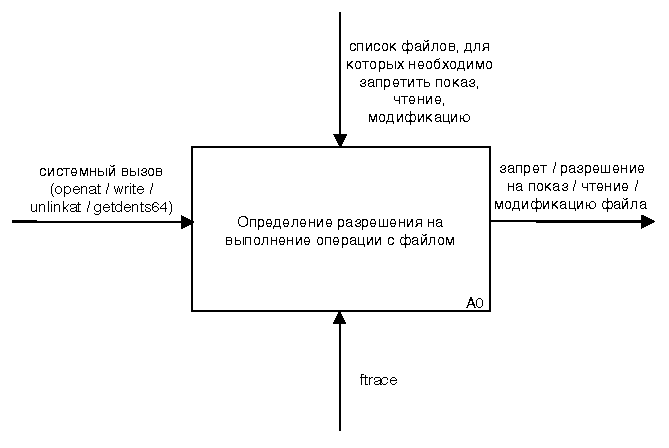
\includegraphics[scale=1.3]{img/idef0_0.pdf}}
	\caption{Диаграмма состояний IDEF0 нулевого уровня}
	\label{fig:idef0}
\end{figure}

\begin{figure}[ph!]
	\center{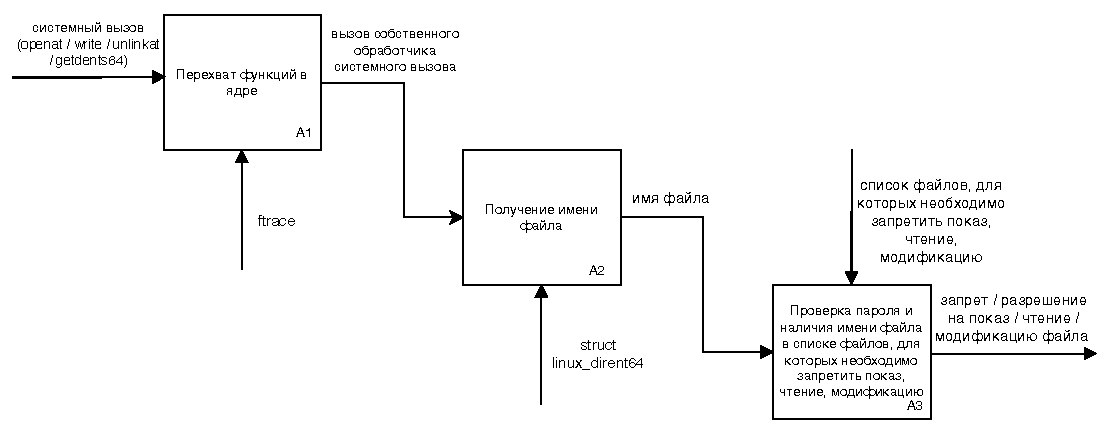
\includegraphics[scale=0.9]{img/idef0_1.pdf}}
	\caption{Диаграмма состояний IDEF0 первого уровня}
	\label{fig:idef1}
\end{figure}

\clearpage

\section{Алгоритм создания символьного устройства}

На рисунке \ref{fig:dev} приведена схема создания символьного устройства.

\begin{figure}[ph!]
	\center{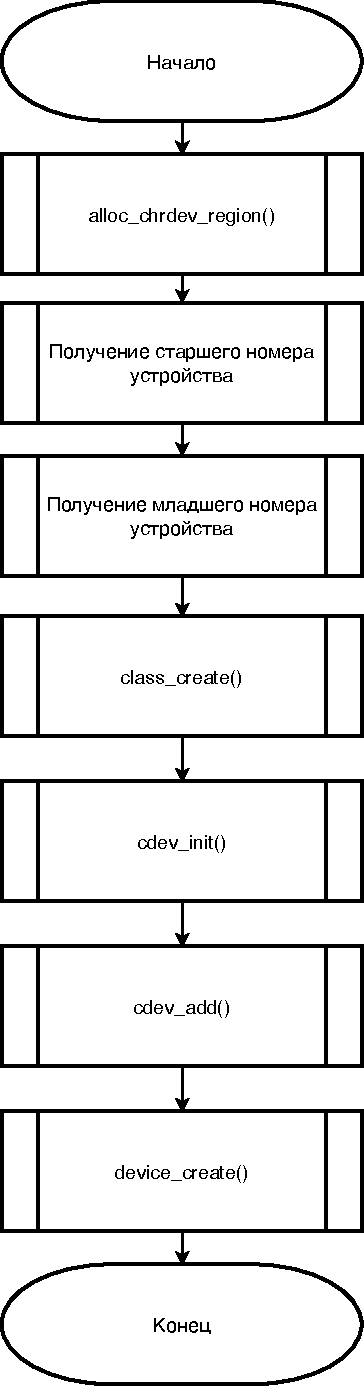
\includegraphics[scale=0.65]{img/cdev.pdf}}
	\caption{Алгоритм создания символьного устройства}
	\label{fig:dev}
\end{figure}

\section{Алгоритм проверки наличия разрешения на модификацию файла}

На рисунке \ref{fig:init} приведена схема алгоритма проверки наличия разрешения на модификацию файла.

\begin{figure}[ph!]
	\center{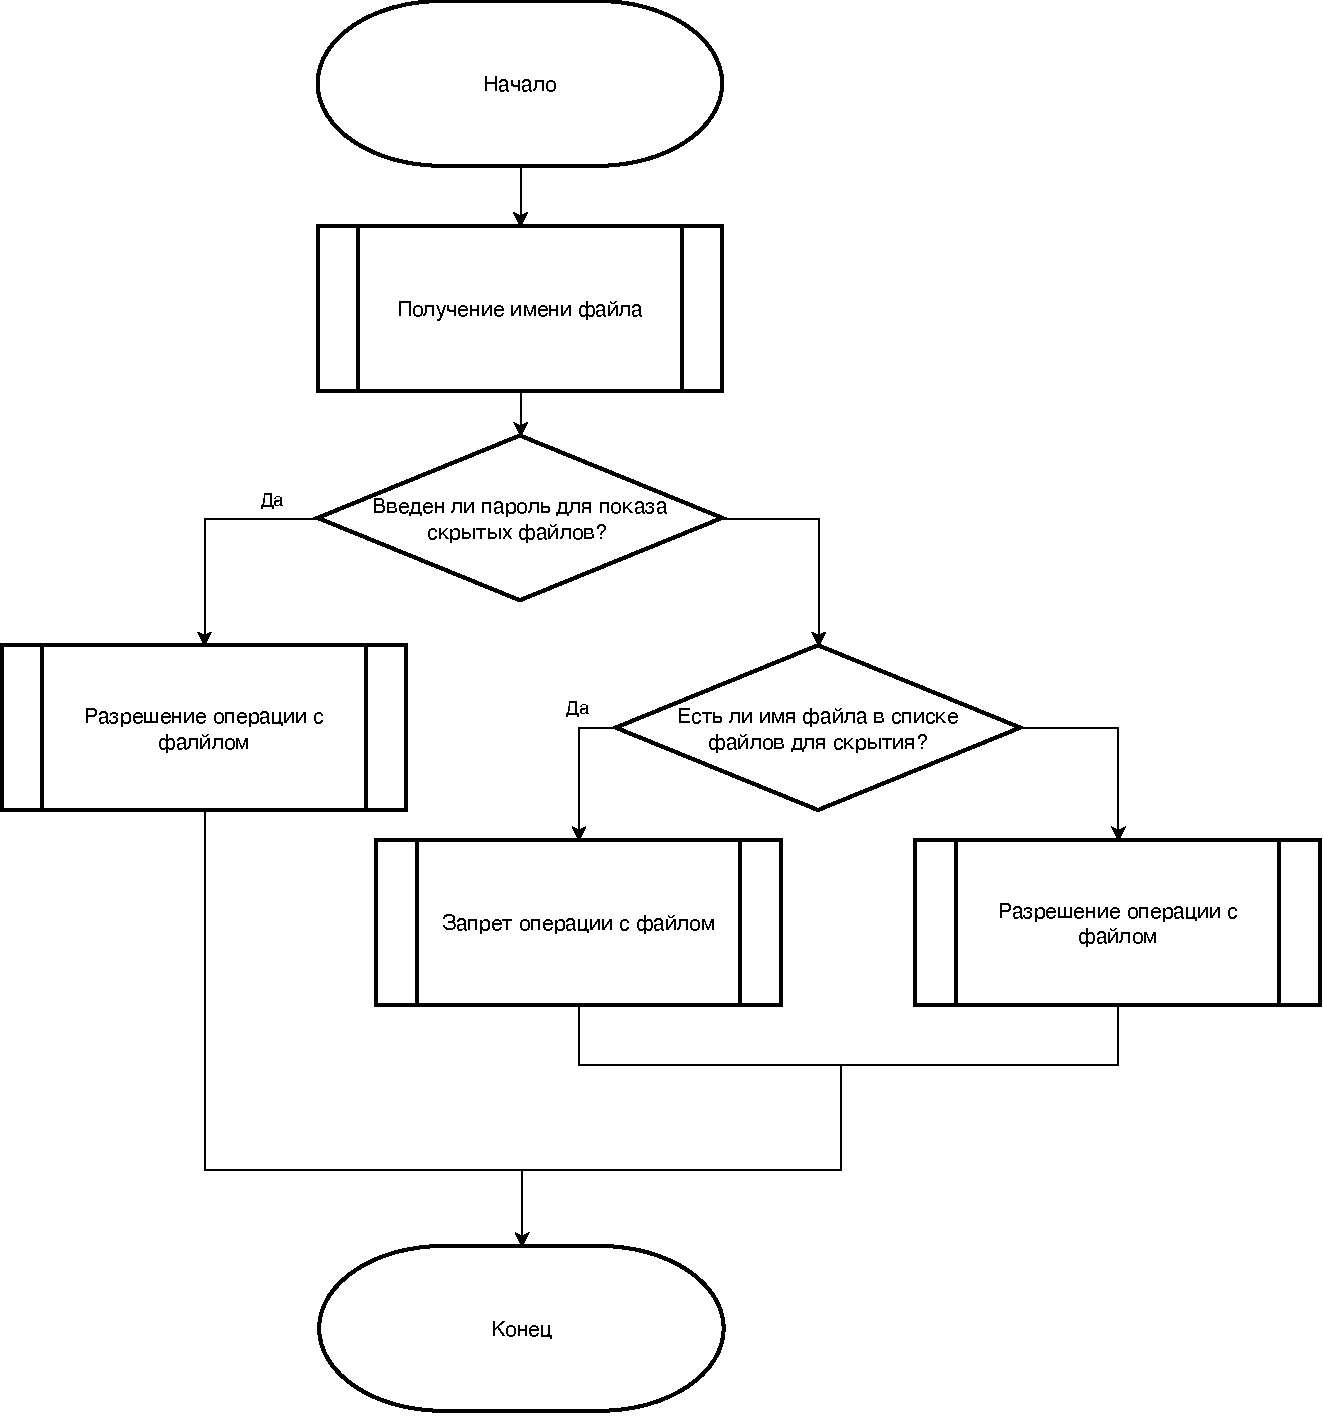
\includegraphics[scale=0.6]{img/check.pdf}}
	\caption{Алгоритм проверки наличия разрешения на модификацию файла}
	\label{fig:init}
\end{figure}

\section{Структура программного обеспечения}

На рисунке \ref{fig:struct} представлена структура программного обеспечения.

\begin{figure}[ph!]
	\center{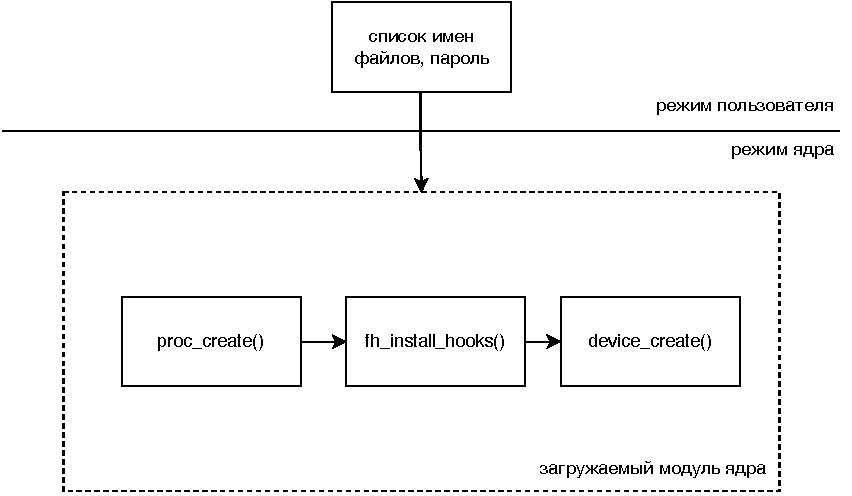
\includegraphics[scale=1]{img/structure.pdf}}
	\caption{Структура программного обеспечения}
	\label{fig:struct}
\end{figure}



